\section{Laboratorium nr 2}

\subsection{Funkcja autokorelacji}
Funkcja (auto)korelacji pozwala uzyskać informacje o podobieństwie dwóch sygnałów w~kolejnych chwilach przesunięcia $\tau$. Może być wykorzystywana do badania okresowości sygnału. Pozwala one na sprawdzenie, jak bardzo dwa sygnały są do siebie podobne. Przyjmuje ona największe wartości dla wartości przesunięcia $\tau$ wynoszącego wielokrotność okresu sygnału. Funkcja autokorelacji można użyć do wyznaczania okresu głosek dźwięcznych mowy czy detekcji odbić w odebranym sygnale echa (echolokacja).

Dla sygnałów dyskretnych funkcja korelacji własnej może być obliczona z~poniższego wzoru:
\begin{equation}\label{lab2/eq/ACF}
	R_{xx}(k) = \sum_{k=\infty}^{\infty} x[n]x[n+k]
\end{equation}
Widać, że powyższa formuła~\ref{lab2/eq/ACF} z wyjątkiem odwrócenia w czasie jednego z sygnałów jest tym samym co splot dwóch wektorów~\ref{lab1/sec/convolution}. 

Do obliczenia wartości funkcji (auto)korelacji w~programie MATLAB, służy funkcja \texttt{xcorr}, która może być wywołana z jednym argumentem albo dwoma argumentami będącymi wektorami próbek analizowanych sygnałów. W pierwszym przypadku zostanie policzona autokorelacja, w drugim natomiast korelacja wzajemna, która pozwala na szukanie podobieństwa pomiędzy dwoma różnymi sygnałami. 

\begin{figure}[hbt!]
	\centering
	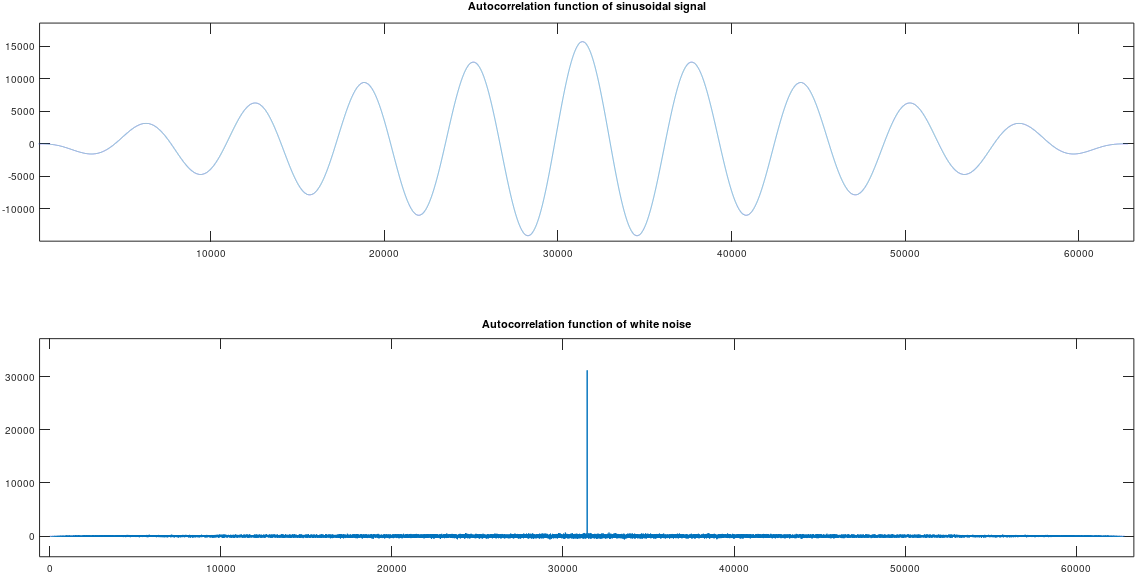
\includegraphics[width=0.9\linewidth]{images/xcorrFunction.png}
	\caption{Przykład funkcji autokorelacji sygnału sinusoidalnego oraz szumu białego.}
	\label{lab2/fig/xcorrFunction}
\end{figure}

Na rysunku~\ref{lab2/fig/xcorrFunction} pokazano wykresy dwóch funkcji autokorelacji odpowiednio sygnału sinusoidalnego oraz szumu białego. W~pierwszym przypadku funkcja autokorelacji ukazuje okresowość badanego przebiegu, posiada powtarzające się oscylacje. Natomiast ze względu na fakt, że kolejne próbki szumu białego są od siebie niezależne (wymusza to również, fakt że są nieskorelowane), funkcja autokorelacji przyjmuje wartości zerowe (z wyjątkiem próbki zerowej, gdzie przyjmuje wartość maksymalną). 

\subsection{Dyskretna transformacja Fouriera}
Przekształcenie Fouriera umożliwia zamianę reprezentacji sygnału z dziedziny czasu na reprezentację w~dziedzinie częstotliwości (inaczej mówiąc jest to transformacja pomiędzy układami współrzędnych). 

Transformacja ta jest narzędziem, które pozwala dowiedzieć się, jakie częstotliwości składowe zawiera sygnał w~dziedzinie czasu poddawany transformacji. Jest ona pewnego rodzaju ,,skanerem'', który bada korelację badanego sygnału z funkcjami sinusoidalnymi i kosinusoidalnymi o różnych częstotliwościach.
\begin{figure}[hbt!]
	\centering
	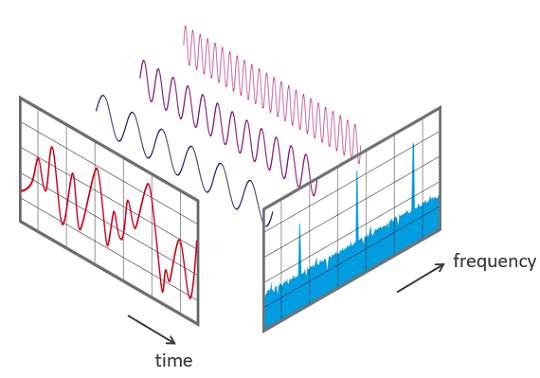
\includegraphics[width=0.9\linewidth]{images/fourierTransform.png}
	\caption{Przykład reprezentacji sygnału w dziedzinie czasu i częstotliwości.}
	\label{lab2/fig/fourierTransform}
	%https://www.allaboutcircuits.com/uploads/thumbnails/Thumnailm7192017.png
\end{figure}

Na rysunku~\ref{lab2/fig/fourierTransform} widać sygnał w~dziedzinie czasu (czerwony wykres). Składa się on z sumy trzech sygnałów sinusoidalnych. W dziedzinie częstotliwości są one reprezentowane jako prążki odpowiedniej częstotliwości poszczególnych składowych. Inaczej mówiąc, jeśli mamy sygnał sinusoidalny o częstotliwości $10~Hz$ to po transformacji Fouriera otrzymamy pojedynczy prążek dla argumentu $10~Hz$ o wysokości równej amplitudzie tej składowej. Jeśli sygnał składa się większej liczby składowych będzie to odwzorowane większą liczbą nie zerowych prążków w dziedzinie częstotliwości. Na rysunku~\ref{lab2/fig/signalInTimeAndFrequencyDomain} przedstawiono sygnał $x(t)$ składający się z~sumy dwóch sygnałów sinusoidalnych o częstotliwościach $50~Hz$ oraz $60~Hz$ i amplitudach odpowiednio $1$ i $0.5$. Na górnej części rysunku~\ref{lab2/fig/signalInTimeAndFrequencyDomain} widać sygnał w~dziedzinie czasu, z którego nie jest łatwo określić jakie składowe zawiera $x(t)$. Na dolnym wykresie natomiast, widać sygnał w~dziedzinie częstotliwości, gdzie wyraźnie są pokazane prążki reprezentujące jego składowe.

\begin{figure}[hbt!]
	\centering
	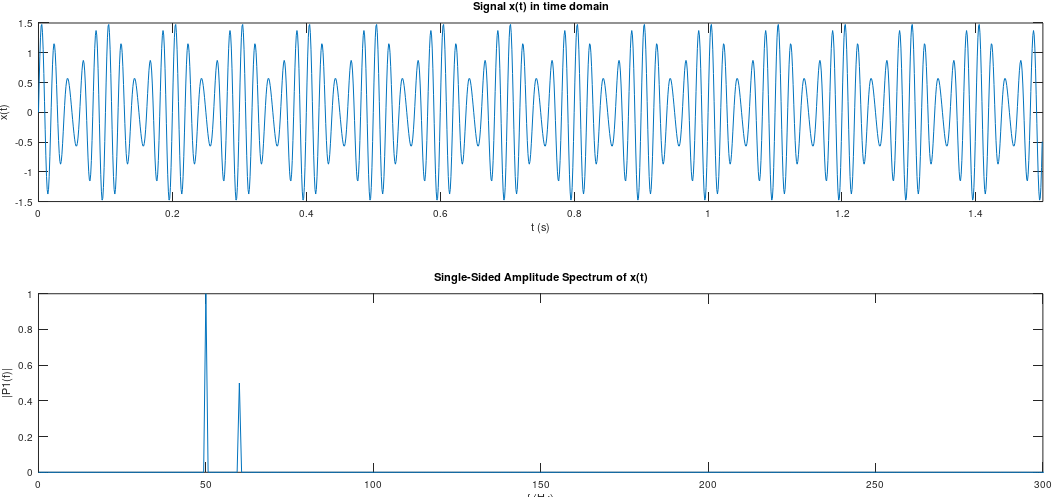
\includegraphics[width=0.9\linewidth]{images/signalInTimeAndFrequencyDomain.png}
	\caption{Przykład reprezentacji sygnału w dziedzinie czasu i po DFT w dziedzinie częstotliwości.}
	\label{lab2/fig/signalInTimeAndFrequencyDomain}
\end{figure}

W przypadku przekształcenia Fouriera konieczne jest realizowanie nieskończonych granic sumowania co jest nierealizowalne w praktycznych zastosowaniach. Dlatego wyznacza się szereg Fouriera dla sygnałów dyskretnych (ang. Discrete Fourier Transform, DFT). Transformacja DFT bierze $N$ próbek przebiegu $x[n]$ i~zwraca w~wyniku wektor $X[k]$ o~długość $N$. Prosta transformacja DFT przyjmuje postać:
\begin{equation}
	X[k] = \frac{1}{N} \sum_{n=0}^{N-1} x[n] e^{-j2\pi \frac{kn}{N}}
\end{equation}
Natomiast odwrotna transformacja DFT może być przedstawiona wzorem:
\begin{equation}
	x[n] = \sum_{k=0}^{N-1} X[k] e^{j2\pi \frac{kn}{N}}
\end{equation}
,gdzie:
\begin{equation}
	e^{-j2\pi \frac{kn}{N}} = [cos(2\pi \frac{kn}{N}) - jsin(2\pi \frac{kn}{N})]
\end{equation}

Z perspektywy tych zajęć laboratoryjnych do wyznaczania transformacji Fouriera, będziemy korzystać z~funkcji \texttt{fft} programu MATLAB/Octave. Pozwala on obliczenie prostej i odwrotnej dyskretnej transformacji Fouriera za pomocą algorytmu szybkiej transformacji Fouriera (ang. Fast Fourier Transform, FFT).

FFT pozwala na efektywne wyznaczenie szeregu Fouriera. Jest to jeden najważniejszych algorytmów jakie zostały wymyślone. Algorytm ten jest wykorzystywany przy analizie sygnałów audio i~obrazów (np. JPEG, MP3, XviD), pozwala na dokonywanie kompresji sygnałów, jest również wykorzystywany przy numerycznym rozwiązywaniu równań różniczkowych. Większość współczesnej komunikacji cyfrowej jest oparta na algorytmie FFT. 

Przy wywołaniu funkcji \texttt{X = fft(x)} z~argumentem będącym wektorem próbek w~dziedzinie czasu zostanie zwrócony wektor liczb zespolonych o takiej samej długości co długość wektora \texttt{x}. Należy jednak mieć na uwadze, że otrzymane widmo jest symetrycznie odbite względem częstotliwości Nyquista\footnote{Częstotliwość Nyquista jest maksymalną częstotliwością sygnału, która może być odtworzona po operacji próbkowania. W~praktyce jest ona równa połowie częstotliwości próbkowania $f_N = \frac{f_S}{2}$.}. Tak więc, po wykonaniu FFT można wziąć do analizy jedynie połowę otrzymanego wektora. Następnie jeśli chcemy, aby wysokość prążków odpowiadała amplitudzie składowych sygnału konieczne jest wykonanie skalowania tzn. podzielenie próbek wektora przez długość tego wektora oraz pomnożeniu go przez dwa. Następnie do narysowania wykresu (za pomocą funkcji \texttt{plot}) należy wziąć moduł otrzymanych liczb zespolonych \texttt{plot(abs(X))}. Przykład zastosowania funkcji \texttt{fft} programu MATLAB/Octave został pokazany na listeningu~\ref{lab2/lst/fftExample}. Podczas zajęć laboratoryjnych zostanie on omówiony krok po kroku.

\begin{lstlisting}[caption=Przykład użycia funkcji \texttt{fft} programu MATLAB/Octave , label=lab2/lst/fftExample]
Fs = 1000;            % Sampling frequency                    
T = 1/Fs;             % Sampling period       
L = 1500;             % Length of signal
t = (0:L-1)*T;        % Time vector

x = 0.7*sin(2*pi*50*t)	
	
X = fft(x);
P2 = abs(X/L);
P1 = P2(1:L/2+1);
P1(2:end-1) = 2*P1(2:end-1);  % multiply by 2 to take into account the fact that we threw out second half of FFTX above

f = Fs*(0:(L/2))/L;
plot(f,P1) 
title('Single-Sided Amplitude Spectrum of x(t)')
xlabel('f (Hz)')
ylabel('|P1(f)|')
\end{lstlisting}



Tak jak zostało wcześniej wspomniane w wyniku operacji FFT zostaje zwrócony wektor $X[k]$ o długość równej liczbie próbek wektora sygnału poddawanego transformacji. Jednocześnie kolejne elementy wektora $X[k]$ odpowiadają kolejnym częstotliwością w przedziale $f\in[0;fs]$, gdzie $fs$ jest częstotliwością próbkowania. Chcąc poprawnie odwzorować argumenty na osi X należy stworzyć wektor wartości od zera do połowy częstotliwości próbkowania.

Funkcja \texttt{fft} zwraca wektor liczb zespolonych $X_{re} + jX_{im}$. Każda liczba zespolona może być opisana za pomocą modułu i fazy. W przypadku \texttt{fft} moduł odpowiada amplitudzie danej składowej przebiegu, natomiast faza przesunięciu w fazie. Dla funkcji $x(t) = 0.5cos(2\pi 5t + \frac{\pi}{3})$ moduł powinien po przeskalowaniu wynieść $0.5$ natomiast faza $60^o$. Tak więc, amplituda może być wyznaczona za pomocą wzoru~\ref{lab2/eq/amplitudeComplex} natomiast faza ze wzoru~\ref{lab2/eq/phaseComplex}. Ze względu na fakt, że funkcja tangens jak i jej odwrotność są zdefiniowane na przedziale $[\frac{-\pi}{2}, \frac{\pi}{2}]$ natomiast w~wyniku operacji \texttt{fft} otrzymujemy liczby zespolone, które mogą posiadać kąt w przedziale $[-\pi, \pi]$, w~celu obliczenia przesunięcia fazowego należy korzystać z funkcji \texttt{atan2()} zamiast standardowej \texttt{atan()}.
\begin{equation}\label{lab2/eq/amplitudeComplex}
	|X[k]| = \sqrt{X^2 _{re} + X^2 _{im}}
\end{equation}

\begin{equation}\label{lab2/eq/phaseComplex}
	\angle X[k] = tan^{-1} \frac{X_{im}}{X_{re}}
\end{equation}

Operację odwrotnej dyskretnej transformaty Fouriera w~programie MATLAB/Octave można zrealizować przy pomocy funkcji \texttt{x = ifft(X)}. Jeśli jako argument tej funkcji przekażemy transformatę Fouriera w~wyniku powinniśmy ponownie otrzymać sygnał w dziedzinie czasu.


\subsection{Wyciek widma i funkcje okien}
Można powiedzieć, że DFT ,,przeszukuje'' sygnał w~celu znalezienia jego składowych. Algorytm wykorzystuje w~tym celu pewną \textbf{skończoną} liczba pasm o~konkretnej szerokości. Zazwyczaj chcemy, aby liczba pasm była jak największa ($\Delta f$ jak najmniejsza), co powoduje większą rozdzielczość transformaty.
\begin{equation}\label{lab2/lst/frequencyResolution}
	\Delta f = \frac{F_s}{N_{FFT}}
\end{equation}

FFT niejawnie zakłada, że sygnał powtarza się po wystąpieniu ostatniej próbki przekazywanego wektora. Jeśli badamy np. funkcję sinus najlepiej jest poddać operacji DFT wielokrotności jej okresu. Inaczej pojawią się nieciągłości, które powodują tzw. wyciek widma. 

Dodatkowo należy wspomnieć, że FFT może ,,znaleźć'' częstotliwości (bez wycieku widma), które idealnie wpasują się w~wielokrotności $\Delta f$. Np. jeśli chcemy zbadać przebieg o częstotliwości $400~Hz$ (częstotliwość próbkowania wynosi $f_s = 8000~Hz$), a długość transformaty wynosi 2048, to nasza składowa powinna znaleźć się w~próbce o indeksie $k = \frac{N\cdot f_k}{f_s} = \frac{2048\cdot400}{8000} = 102.4$. Oczywiście, jako że $k$ jest indeksem elementu naszej transformaty to indeks ten powinien być dodatnią liczbą całkowitą. W tym przypadku energia z tej składowej zostanie ,,rozlana'' i znajdzie się w~elementach wektora o indeksach $102$ oraz $103$.

Aby ograniczyć wyciek widma, należy pomnożyć sygnał z~funkcją okna. Taka operacja powoduje, że na początku i końcu wektora, sygnał ulega wygaszeniu i~nie pojawiają się nieciągłości w~sygnale. 
\begin{figure}[hbt!]
	\centering
	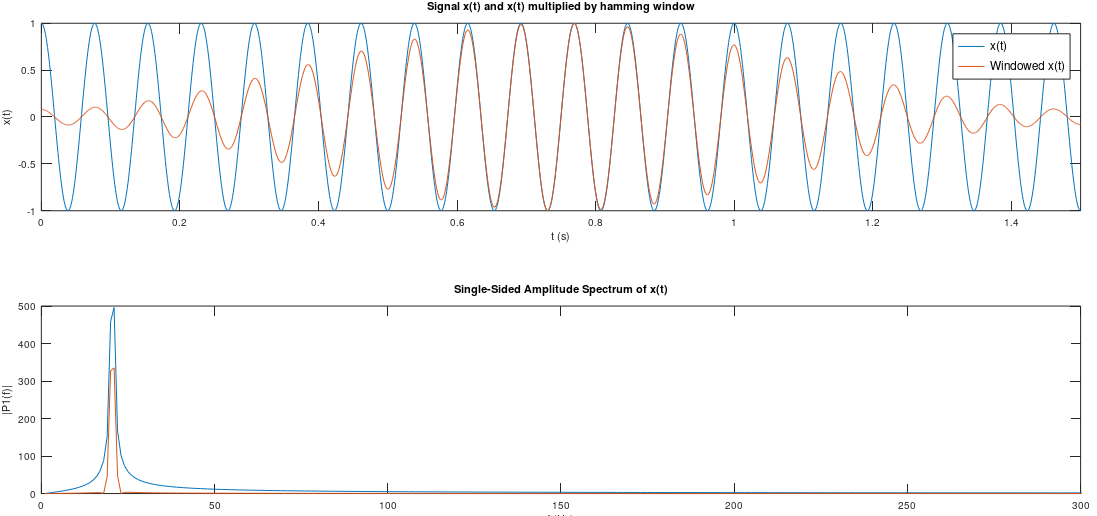
\includegraphics[width=0.9\linewidth]{images/spectralLeakage.png}
	\caption{Przykładowy wyciek widma spowodowany złą długością wektora transformaty Fouriera oraz zmniejszenie niepożądanego efektu za pomocą wymnożenia sygnału przez okno Hamminga.}
	\label{lab2/fig/spectralLeakage}
\end{figure}
Istnieje wiele typów funkcji okien (Hanna, Hamminga, Blackmana, Kaisera), które charakteryzują się szerokością listka głównego i tłumieniem listków bocznych, a wybór jednego z nich ma wpływ na kształt otrzymywanego widma i oferowaną przez niego rozdzielczość. Poniżej został pokazany sposób utworzenia wektora okna Hamminga w~programie MATLAB/Octave i~jego wymnożenie przez sygnał sinusoidalny $x(t)$~\ref{lab2/lst/hammingWindow}. Na rysunku~\ref{lab2/fig/spectralLeakage} pokazano natomiast funkcję $x(t)$ oraz funkcję $x(t)$ wymnożoną przez okno Hamminga. Na górnym wykresie w dziedzinie czasu widać funkcja wymnożona przez okno na końcach zbiega do zerach. Natomiast na wykresie w~dziedzinie częstotliwości,  można zaobserwować, że wykorzystanie okna drastycznie zmniejszyło niepożądany efekt wycieku widma.    
\begin{lstlisting}[caption=Wymnożenie sygnału $x(t)$ przez okno Hamminga , label=lab2/lst/hammingWindow]
	wnd = hamming(length(x));
	xWnd = x'.*wnd;
	Y = fft(xWnd);
\end{lstlisting}


\subsection{Zadania}
%\subsubsection{Aproksymacja przebiegu czasowego za pomocą szeregu Fouriera}
%Za pomocą szeregu Fouriera wyznacz współczynniki $a_n$ oraz $b_n$ aproksymujące podane poniżej funkcje $x(n)$:
%\begin{itemize}
%	\item $y(t) = 1/T \cdot t$, dla $t \in [0,T] $
%	\item $y(n) = \begin{cases} 1, & \mbox{dla } t\in [0,\frac{T}{2}] \\ -1, & \mbox{dla } t\in [\frac{T}{2}, T] \end{cases}$ 
%	\item $y(n) = \begin{cases} \frac{2}{T}\cdot t, & \mbox{dla } t\in [0,\frac{T}{2}] \\ \frac{-2}{T} t, & \mbox{dla } t\in [\frac{T}{2}, T] \end{cases}$ 
%\end{itemize}
%Narysuj wykres funkcji dla $N$ wynoszącego odpowiednio: $2$, $5$ oraz $20$. Wraz ze zwiększaniem się liczby współczynników powinna się poprawiać dokładność aproksymacji funkcji $y(t)$.

\subsubsection{Badanie okresowości sygnału na podstawie funkcji autokorelacji}
Dokonaj analizy za pomocą funkcji autokorelacji przebiegu czasowego postaci: $x(t) = sin(2\pi10t) + 3n(t)$, gdzie $n$ jest szumem białym o rozkładzie normalnym i~odchyleniu standardowym równym $3$. Narysuj na współdzielonym wykresie:
\begin{itemize}
	\item przebieg sygnału $x(t)$ w dziedzinie czasu,
	\item funkcję autokorelacji za pomocą funkcji programu MATLAB/Octave \texttt{xcorr(x)}.
\end{itemize}

Zwróć uwagę, że na wykresie funkcji autokorelacji dużo łatwiej można zaobserwować okresowość sygnału wejściowego. 

\subsubsection{Wyznaczenie dyskretnej transformacji Fouriera}
Wyznacz transformaty Fouriera następujących sygnałów:
\begin{itemize}
	\item $y(t) = cos(2\pi10t)$,
	\item $y(t) = cos(2\pi10t + \frac{\pi}{6})$,
	\item $y(t) = cos(2\pi10t) + cos(2\pi20t) + cos(2\pi30t)$,
	\item $y(t) = cos(2\pi10t) + n(t)$ (funkcja sinus z dodanym szumem białym o rozkładzie normalnym),
	\item przebiegu prostokątnego,
	\item szumu białego o rozkładzie równomiernym i normalnym.
\end{itemize}

\subsubsection{Usunięcie szumów z sygnału z wykorzystaniem FFT}
Stwórz sygnał $x(t) = cos(2\pi10t) + cos(2\pi20t)$ o~takiej długości, aby składowa o niższej częstotliwości zawierała najmniej kilka okresów. Następnie dodaj do niego szum o rozkładzie normalnym (długość wektora zawierającego szumy powinna być taka sama jak długość wektora zawierająca sygnał, możesz posłużyć się funkcją \texttt{length()} albo \texttt{size()} w~celu pobrania długości wektora/tablicy). 

Przygotuj współdzielony wykres (\texttt{subplot(2,1,2)}). Na górnym wykresie narysuj przebieg sygnału $x(t)$ za pomocą funkcji \texttt{plot(t,x)}. Następnie wyznacz dyskretną transformatę Fouriera tego sygnału. Wyzeruj wszystkie elementy wektora (wartości dla których \texttt{abs(X) > threshold}), które nie przekraczają zdefiniowanego progu np. $100$, nie jest konieczne wykonywanie normalizacji/skalowania transformaty Fouriera na tym etapie. Dalej dla tak zmanipulowanego wektora $X[k]$ oblicz odwrotną transformatę Fouriera (\texttt{ifft(X)}). Wynik przedstaw na utworzonym wcześniej współdzielonym wykresie. 

\subsubsection{Rozdzielczość transformaty Fouriera}
Zazwyczaj obliczanych jest podczas dyskretnej transformaty Fouriera tyle prążków widma, ile próbek ma sygnał. Należy jednak pamiętać, że im więcej otrzymamy w~wyniku DFT prążków tym lepiej będzie odwzorowane faktyczne widmo sygnału. Stwórz sygnał składający się z dwóch składowych o~częstotliwościach znajdujących się blisko siebie np. $50~Hz$ oraz $60~Hz$. Wywołując funkcję \texttt{fft()} z~drugim dodatkowym parametrem możemy zmieniać długość wektora transformaty (\texttt{fft(x,n)} zwróci nam \texttt{n} elementową transformatę). Sprawdź jaka jest najmniejsza wartość \texttt{n}, która pozwoli na rozróżnienie dwóch prążków stworzonego przed chwilą sygnału $x[n]$

\subsubsection{Zmniejszenie efektu wycieku widma przez zastosowanie okna Hamminga}
Stwórz sygnał o~częstotliwości np. $13~Hz$ i~o~długości $1500$ próbek. Częstotliwość próbkowania należy ustawić tak, aby spowodować wyciek widma np. $f_s = 1000$. Oblicz widmo utworzonego sygnału i~narysuj go na wykresie. Następnie wymnóż ten sygnał przez okno Hamminga (listening~\ref{lab2/lst/hammingWindow}), o takiej samej długości co sygnał i ponownie wyznacz widmo. Użyj wyrażenie \texttt{hold on} i ponownie narysuj wykres widma (tym razem sygnału wymnożonego przez okno). Efekt wycieku widma w~drugim przypadku powinien być zniwelowany. 

\newpage